% !TeX root = ../index.tex
\documentclass[../index.tex]{subfiles}

\begin{document}
    \section{Wykład}
        \subsection{Konstruowanie modelu gwiazdy}
            Metoda konstruowania modelu wnętrza gwiazdy bazuje na równaniach zachowania: masy, energii i pędu. Na ich podstawie oraz założenie, że gwiazda jest zbiorem koncentrycznych powłok sferycznych o grubości \(dr\) konstruuje się pięc równań różniczkowych:
            \begin{align}
                \frac{dP(r)}{dr} &=  -\rho(r)G \frac{M(r)}{r^2 } \text{ — zasada zachowania pędu (równanie równowagi termodynamicznej)}\\
                \frac{dM(r)}{dr} &=  4\pi r^2 \rho(r) \text{ — zasada zachowania masy} \\
                \frac{dL(r)}{dr} &= 4\pi r^2 \rho(r)\varepsilon(\rho,T) \text{ — zasada zachowania energii}\\
                \frac{dT(r)}{dr} &= - \frac{3}{16\pi} \frac{\kappa}{\sigma_B T^3 }\frac{L(r)}{r^2 } \text{ — zasada zachowania energii (transport promienisty)} \\
                \frac{dT(r)}{dr} &= - \frac{\mu m_u}{\kappa} \autoround{1 - \frac{1}{\gamma(\rho,T)}} G \frac{M(R)}{r^2 } \text{ — zasada zachowania energii (transport konwektywny)} 
            \end{align}
            gdzie \(\rho\) – gęstość, \(\varepsilon\) – ilość energii wydzielonej w reakcjach termojądrowych w jednostce czasu na jednostkę objętości, \(\kappa\) – współczynnik absorbcji ośrodka, \(\mu\) – średni ciężar cząsteczkowy, \(m_u\) – atomowa jednostka masy. Czwarte i piąte równanie stosuje się zamiennie w zależności od tego jaki typ transportu energii dominuję – promieniowanie czy konwekcja. Warunkami brzegowymi są wartości parametrów na powierzchni gwiazdy (możliwe do zaobserwowania bezpośrednio):
            \begin{align*}
                T(R) &=  T_\text{eff} \\
                P(R) &= P_s \\
                L(R) &= L \\
                M(R) &=  M
            \end{align*}
            W praktyce tworzenie modelu polega na wyliczaniu kolejnych wartości każdego z parametrów na kolejnych powłokach (\(dr\) skończenie małe?).
        \subsection{Części Słońca}
            Na podstawie przeprowadzonych modelowań, we wnętrzu Słońca wyróżnia się trzy zasadnicze części:
            \begin{enumerate}
                \item \textbf{Jądro} – dla \(r \leq 0.3 R_\odot\). Temperatura przekraczająca 7 milionów kelwinów umożliwia zachodzenie reakcji termojądrowych syntezy helu. Skład chemiczny jądra znacznie różni się od składu fotosfery – to wynik procesów termojądrowych, które obniżają stężenie wodoru na rzecz helu.
                \item \textbf{Otoczka promienista} – dla \(r\in\{0.3 R_\odot, 0.72 R_\odot\}\). Nie zachodzą tu reakcje termojądrowe, a transport energii zachodzi w formie promienistej.
                \item \textbf{Otoczka konwektywna} zajmuje zewnętrzną powłokę słońca. Stosunkowo niska temperatura (2 mln \(K\)) powoduje wzrost współczynnika absorbcji i blokuje większość transportu promienistego. Ta warstwa zawiera około \(2\%\) masy słońca i około \(\frac{2}{3}\) jego objętości.
            \end{enumerate} 
            Oczywiście nie istnieje jeden właściwy model Słońca. Różne podejścia różnią się pewnymi szczegółami.
        \subsection{Zależność budowy gwiazdy od jej masy}
            W celu stworzenia modelu, który nie zaniedbuje zmiany składu chemicznego w wyniku starzenia się gwiazdy wprowadza się pojęcie \textbf{ZAMS} tzn. gwiazd ciągu głównego o zerowym wieku. Im gwiazda bardziej masywna tym cieplejsza i, oprócz wyjątków, mnie gęsta. Wyższa temperatura przekłada się na większe tempo zachodzenia reakcji termojądrowych. Gdy porówna się słońce z dziesięciokrotnie cięższą gwiazdą, to podaż energii w centralnej części tej drugiej jest kilka tysięcy razy większa. Zależność gęstości od temperatury obrazuje poniższy wykres:
            \begin{center}
                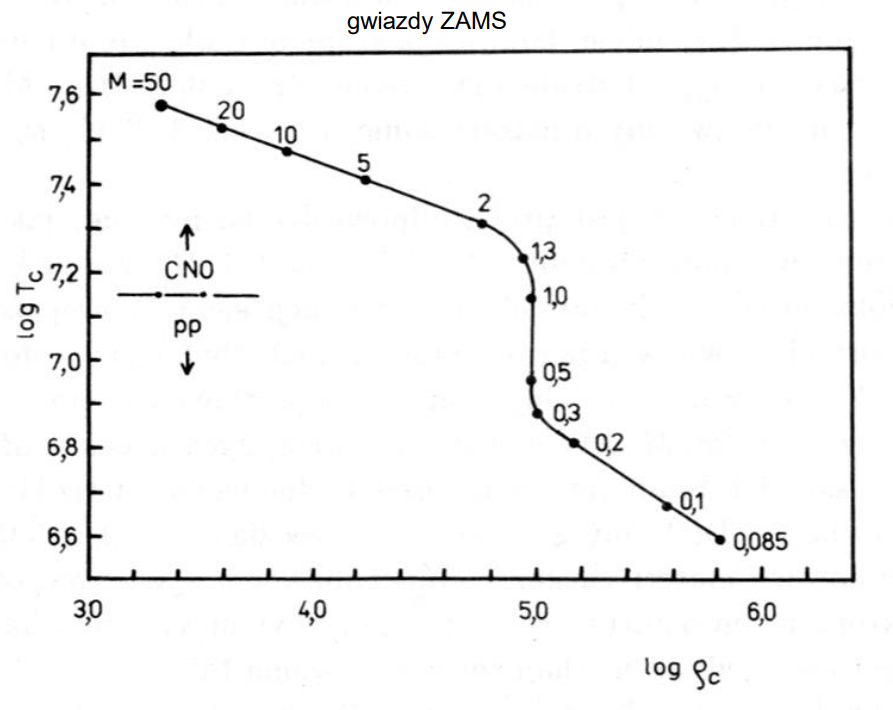
\includegraphics[width=13cm]{images/temperatura-gestosc-relacja.png}
            \end{center}
            Jak widać gęstość spada wraz ze wzrostem temperatury dla niemal wszystkich mas — jedynie te z przedziału od \(0.3 M_\odot\) do \(1.4 M_\odot\) nie zmieniają swojej gęstości wraz ze wzrostem temperatury. Wyjaśnienia tego efektu można doszukiwać się na poniższym wykresie:
            \begin{center}
                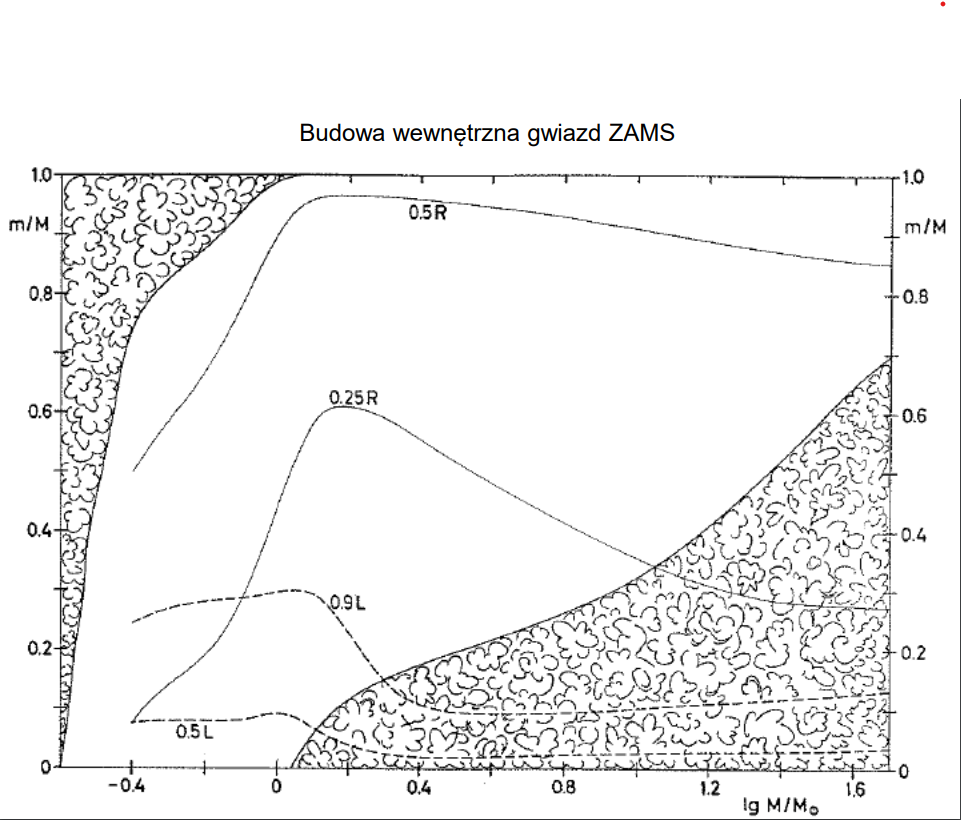
\includegraphics[width=15cm]{images/budowaGwiazdZAMS.png}
            \end{center}
            Powyżej białe tło oznacza dominacje transportu promienistego, a tło ,,kłaczkowate'' dominacje transportu konwektywnego. Na osi OX mamy stosunek masy gwiazdy do masy Słońca, a na osi OY takie położenia w gwieździe, że np. 0.5 oznacza, że ,,pod stopami'' znajduje się \(50\%\) masy gwiazdy. Linie \(0.5 L\), \(0.9 L\) wyznaczają obszary, które generują odpowiednio \(50\%\) i \(90\%\) światłości gwiazdy, a \(0.25R\) i \(0.5R\) odpowiednio \(\frac{1}{4}\) i \(\frac{1}{2}\) promienia gwiazdy. Jak widać istnieją dwa obszary występowania transportu konwekcyjnego : 
            \begin{itemize}
                \item w przypadku gwiazd masywnych \(M > 1.4 M_\odot\) konwekcja obejmuje jądro, ponieważ transport promienisty nie jest w stanie odprowadzić całkowitej tworzącej się tam energii. Dla gwiazd o jeszcze większej masie konwekcja obejmuje również fragment otoczki przylegającej do jądra.
                \item w przypadku gwiazd o mniejszych masach konwekcja pojawia się w zewnętrznej części otoczki. Im mniejsza masa tym konwekcja sięga coraz głębiej, aż dla \(M < 0.3 M_\odot\) gwiazda staje się całkowicie konwektywna. W tym przypadku kownekcja wynika z wysokiej nieprzezroczystości ośrodka.
            \end{itemize}
            Jak widać nietypowe zachowanie dotyczy gwiazd o masach z przedziału \(0.3\)-\(1.4 M_\odot\), a więc z transportem promienistym w obszarze jądra.
        \subsection{Mierzenie wnętrz gwiazdowych}
            Mimo, że nieprzezroczyste dla fotonów, wszystkie warstwy słońca są przezroczyste dla neutrin – słabo oddziałujących z materią cząstek elementarnych, które powstają w procesach termojądrowych. Na szczęście neutrina da się rejestrować różnorakimi detektorami. Zwykle wymagają one ogromnych przestrzeni (bo słabe oddziaływanie) i są umieszczone głęboko pod ziemią (żeby szumy z powierzchni Ziemi nie wpływały na pomiary – tylko neutrina dotrą tak głęboko). Jednak pierwsze pomiary neutrin bardzo mocno różniły się od przewidywań teoretycznych. Problem ten nazwano \textbf{deficytem neutrin słonecznych}. Jednakże do tych pomiarów użyto detektorów mogących mierzyć jedynie \textbf{neutrina elektronowe} (tylko takie powstawały w wyniku reakcji termojądrowych, więc wątpliwości były uzasadnione). Użycie detektorów oddziałujących także z neutrina \textbf{mionowymi} i \textbf{taonowymi} wykazywały zgodność z teoretycznymi wyliczeniami. Efekt ten wynika z faktu, że mimo tego, że wszystkie neutrina powstałe w słońcu to neutrina elektronowe, to mogą one przekształcać się w pozostałe dwa typy. Zjawisko to nosi miano \textbf{oscylacji neutrin} i jest dowodem na masowość tychże.
        \subsection{Chromosfera}
            Innym testem na poprawność modeli wnętrz gwiazdowych są obserwacje wskazujące na obecność \textbf{chromosfery} tylko w przypadku niektórych typów gwiazd ciągu głównego. Chromosferę można zaobserwować bezpośrednio na Słońcu oraz dowiedzieć się o jej istnieniu na podstawie analizy widma. Chromosfera to obszar atmosfery słońca, w którym temperatury rośnie ze wzrostem odległości od powierzchni (zamiast maleć). Jej obecność jest słabo widoczna w widmie ze względu na znacznie niższą gęstość. Jednakże w zakresach promieniowania innych niż widzialne, nieprzezroczystość atmosfery słońca jest znacznie większa i promieniowanie wydostaje się swobodnie dopiero na poziomie chromosfery (co umożliwia jej obserwacje). \\
            Chromosfera występuje jedynie dla gwiazd ciągu głównego o masie mniejsze niż \(1.4 M_\odot\). Gwiazdy te charakteryzuje obecność warstwy konwektywnej zlokalizowanej przy powierzchni gwiazdy. Ruchy materii towarzyszące konwekcji generują szerokie spektrum fal dźwiękowych. Niektóre z nich propagują na zewnątrz atmosfery i w ośrodku o malejącej gęstości deformują się w fale uderzeniowe, których energia przekształcana jest w temperature ośrodka.
\end{document}